\documentclass[11pt,a4paper]{article}

% ------------------------------------------------------------
% Pacotes (mesmo preâmbulo da proposta, report/report.tex)
% ------------------------------------------------------------
\usepackage[utf8]{inputenc}
\usepackage[T1]{fontenc}
\usepackage[brazil]{babel}
\usepackage{lmodern}
\usepackage{microtype}
\usepackage{amsmath,amssymb}
\usepackage{enumitem}
\usepackage{geometry}
\usepackage{titlesec}
\usepackage{booktabs}
\usepackage{graphicx}
\usepackage{caption}
\usepackage{hyperref}

% ------------------------------------------------------------
% Layout
% ------------------------------------------------------------
\geometry{top=1.8cm, bottom=1.8cm, left=1.9cm, right=1.9cm}

\setlength{\parindent}{0pt}
\setlength{\parskip}{3pt}
\setlist[itemize]{leftmargin=1.35em, itemsep=0.8pt, topsep=2pt, parsep=0pt}
\setlist[enumerate]{leftmargin=1.55em, itemsep=0.8pt, topsep=2pt, parsep=0pt}

\titleformat{\section}{\bfseries\normalsize}{}{0pt}{}
\titlespacing*{\section}{0pt}{7pt}{2pt}

\captionsetup{font=small, labelfont=bf, skip=3pt}
\setlength{\textfloatsep}{8pt}
\setlength{\floatsep}{6pt}

\hypersetup{colorlinks=true, linkcolor=black, urlcolor=blue}

\newcommand{\repo}{https://github.com/annwith/gender-representation-networks}
\newcommand{\dados}{\repo/tree/main-run-results/data/graphml}

% ------------------------------------------------------------
% Documento
% ------------------------------------------------------------
\begin{document}

\begin{center}
    {\large\bfseries MO438 -- Redes Complexas: Entrega Parcial}\\[2pt]
    Da rede lexical à rede contextual: reorganização das representações
    internas de Transformers com Redes Complexas\\[2pt]
    Juliana Midlej do Espirito Santo (RA 200208)
\end{center}

\vspace{-2mm}

% ============================================================
\section*{1. Introdução}

Na entrada de um Transformer, todas as ocorrências de um mesmo token têm o mesmo
\textit{embedding}; ao atravessar as camadas, essas representações incorporam o
contexto e se reorganizam. O projeto descreve essa transformação como uma sequência de
redes complexas sobre \textbf{os mesmos vértices}: cada vértice é uma
\textit{ocorrência} de um token em um texto, e cada ocorrência se liga às $k$ ocorrências
mais semelhantes a ela. Comparando as redes camada a camada, queremos medir quanto a
vizinhança deixa de ser determinada pela identidade do token e passa a refletir o
contexto (perguntas P1--P4 da proposta: reorganização local e global, camadas em que ela
se concentra, comunidades contextuais e separação das ocorrências de um mesmo token).

\textbf{Dados do projeto:} \url{\repo}. As quatro redes analisadas aqui estão em
GraphML em \href{\dados}{\texttt{data/graphml/}} (ramo \texttt{main-run-results}); o
script que as gera, junto com esta análise, é
\texttt{scripts/partial\_delivery/export\_networks.py}.

% ============================================================
\section*{2. Origem dos dados e construção das redes}

As redes são originais, construídas por nós; não foram baixadas de um repositório de
redes. As duas fontes usadas são públicas:
\begin{itemize}
    \item \textbf{Textos:} Wikipédia em português (\url{https://pt.wikipedia.org}, licença
    CC BY-SA), obtida pela API MediaWiki a partir de 8 categorias temáticas (física,
    biologia, economia, política, computação, música, futebol, geografia). A identificação
    e a revisão de cada artigo estão em \texttt{data/corpus/manifest.csv}, o que permite
    baixar de novo exatamente o mesmo texto.
    \item \textbf{Modelo:} \href{https://huggingface.co/Qwen/Qwen3-4B-Base}{Qwen3-4B-Base}
    (Hugging Face, 36 blocos, revisão \texttt{906bfd4}), cujo \textit{tokenizer} também
    define os tokens.
\end{itemize}

\textbf{Coleta.} Em cada tema, uma busca em largura percorre as subcategorias até a
profundidade 2 e para em 600 títulos, entre os quais são sorteados 150 artigos. Como a API
lista as subcategorias em ordem alfabética, o corte não é aleatório: os oito temas atingiram
o limite tendo aberto só parte das subcategorias (de 7 de 79 em computação a 98 de 439 em
música), e, nas listas de subcategorias por país de música e futebol, só as do começo do
alfabeto foram abertas. Os temas são, portanto, ``artigos próximos da categoria raiz'', e não
a área inteira, o que basta para o uso que fazemos deles (temas bem separados). Para
reforçar sentidos raros dos alvos (\textit{nota} como cédula, \textit{banco} de areia),
entram também 16 categorias extras ligadas a temas (profundidade 1, até 60 artigos cada;
\texttt{configs/experiment.yaml}), com 475 dos 1.172 artigos e 38\% dos vértices.

\textbf{Vértices.} Cada vértice é uma \textit{ocorrência}: um token do \textit{tokenizer} do Qwen3, que pode
ser só um pedaço de palavra, numa posição de um parágrafo. A rede não cobre o corpus inteiro
(17.066 parágrafos de 2.153 artigos). São 13.606 ocorrências de 2.864 tipos de token, em
3.230 parágrafos de 1.172 artigos, escolhidas em quatro estratos com no máximo 50
ocorrências por tipo (\texttt{configs/experiment.yaml}, semente 438):
\begin{itemize}
    \item \textbf{Núcleo} (10.020 vértices, 74\%): em cada um dos 8 temas, sorteamos 5
    artigos e 2 parágrafos de cada um, 80 parágrafos ao todo (0,5\% do corpus). Nesses
    parágrafos \emph{todos} os tokens são vértices: palavras, fragmentos, números e
    pontuação. Das 11.935 ocorrências, o teto retira ao acaso 1.915, de 25 tipos frequentes
    (vírgula, ponto, \textit{de}, \textit{que}, \textit{-ão}\ldots).
    \item \textbf{Alvos} (477): 11 palavras polissêmicas (\textit{banco}, \textit{campo},
    \textit{nota}\ldots), com uma cota por tema de sentido (\textit{banco} em economia,
    computação e geografia). \textit{Planta} saiu da amostra por não chegar a 10
    ocorrências em dois temas.
    \item \textbf{Controles} (277): 6 palavras frequentes sem ambiguidade forte
    (\textit{ano}, \textit{água}\ldots), com cotas iguais às dos alvos.
    \item \textbf{Multitemáticas} (2.832): 150 palavras de conteúdo presentes em ao menos
    3 temas, até 20 ocorrências cada.
\end{itemize}
Os três últimos estratos sorteiam palavras inteiras nos demais parágrafos, no máximo uma
ocorrência da mesma palavra por parágrafo e três por artigo. Nesses 3.150 parágrafos, só as
posições sorteadas são vértices, e o resto do texto serve apenas de contexto (2.762 deles
têm um único vértice). O núcleo dá uma amostra de texto corrido. Os demais estratos existem
porque 80 parágrafos quase não repetem palavras de conteúdo, e sem repetição não há como
comparar a mesma palavra em contextos diferentes. Por construção, todos os fragmentos,
números, sinais de pontuação e palavras funcionais vêm do núcleo. No total são 6.583
palavras inteiras, 6.345 fragmentos de palavra (início ou continuação), 351 números e 327
sinais de pontuação. Como o núcleo reúne três quartos dos vértices, as medidas globais
descrevem sobretudo texto corrido. O sorteio de 10 parágrafos por tema, feito com uma única
semente, pesa no vocabulário: 2.780 dos 2.864 tipos aparecem no núcleo.

\textbf{Extração dos vetores.} Cada parágrafo é tokenizado, recebe na frente o separador de documentos
\texttt{<|endoftext|>} e passa sozinho pelo Qwen3, numa chamada própria e sem \textit{cache}:
o modelo não vê o título nem os outros parágrafos do artigo, e não há contexto compartilhado
entre parágrafos ou artigos. A sequência é cortada logo depois da última ocorrência sorteada
no parágrafo. Dentro do modelo, cada posição carrega um vetor de dimensão 2560 (o fluxo
residual), que cada um dos 36 blocos atualiza com atenção e MLP; como a atenção é causal, o
vetor de uma posição depende só do seu token e dos anteriores. O vetor \textbf{lex} não passa
pelo modelo: é a linha do token na matriz de \textit{embeddings}, igual para todas as
ocorrências do token. \textbf{L01}, \textbf{L18} e \textbf{L36} são capturados durante a
chamada por \textit{hooks} do PyTorch nos blocos 1, 18 e 36: quando o bloco termina, o
\textit{hook} recebe a sua saída bruta (antes da normalização final), com uma linha por
posição, e guarda só as linhas das posições sorteadas. Assim, as ocorrências de um mesmo
parágrafo saem da mesma chamada, cada uma lida na sua posição, com o mesmo resultado que
teriam em chamadas separadas. As linhas
são reunidas numa matriz $13.606\times2560$ por representação.

\textbf{Arestas.} Cada ocorrência $i$ recebe um vetor $x_i$ e escolhe, entre as outras 13.605
ocorrências (de qualquer parágrafo, artigo ou tema), os $k=10$ vizinhos de maior
similaridade de cosseno (calculada em \texttt{float64}). O modelo nunca processa dois
parágrafos juntos: a comparação entre ocorrências de parágrafos diferentes acontece só no
espaço dos vetores. As quatro redes diferem
apenas em $x_i$: \textbf{lex}, o \textit{embedding} de entrada do token (ocorrências do
mesmo token são idênticas, e os empates são desfeitos ao acaso, semente 0); \textbf{L01},
\textbf{L18} e \textbf{L36}, a saída dos blocos 1, 18 e 36 (inicial, intermediário e
final). A relação k-NN é direcionada; as redes entregues e analisadas são as versões
\textbf{não direcionadas por união}, com aresta $\{i,j\}$ quando $j$ está entre os vizinhos
de $i$ ou $i$ entre os de $j$. Por isso todo vértice tem grau $\ge k$. Usamos a união por
dois motivos. Primeiro, clusterização, distâncias, componentes e comunidades são definidas
para grafos não direcionados; na versão direcionada, a maioria dos pares não tem caminho
(82\% dos pares ordenados em lex), e a distância média fica infinita. Segundo, a união
preserva todas as relações de vizinhança, enquanto a versão mútua (aresta só quando $i$ e
$j$ se escolhem) descartaria de 39\% a 56\% dos arcos e fragmentaria lex em 1.497
componentes. A versão direcionada continua sendo usada para os graus de entrada
(\textit{hubs}) e a reciprocidade.

\textbf{Arquivos.} \texttt{\textit{rede}\_k10\_union.graphml}, com \textit{rede} em
\texttt{lex}, \texttt{L01}, \texttt{L18} e \texttt{L36} (cerca de 16\,MB cada). Cada vértice traz o token, a palavra de origem, o tema, o artigo, o contexto
textual e as medidas desta análise (grau, clusterização local, componente e comunidade
Leiden). Todas as métricas abaixo foram calculadas com \texttt{igraph} a partir dos
próprios arquivos GraphML relidos do disco.

% ============================================================
\section*{3. Análise inicial}

\begin{table}[h]
\centering
\small
\caption{Métricas das quatro redes ($k=10$, união).
$^\ast$Calculadas de forma exata sobre todos os pares de vértices da maior componente.}
\label{tab:metricas}
\begin{tabular}{lrrrr}
\toprule
Métrica & lex & L01 & L18 & L36 \\
\midrule
Vértices & 13.606 & 13.606 & 13.606 & 13.606 \\
Arestas & 102.656 & 97.061 & 94.739 & 106.307 \\
Grau médio & 15,09 & 14,27 & 13,93 & 15,63 \\
Grau mínimo / máximo & 10 / 37 & 10 / 60 & 10 / 55 & 10 / 247 \\
Densidade ($\times 10^{-3}$) & 1,109 & 1,049 & 1,024 & 1,149 \\
Transitividade (clusterização global) & 0,531 & 0,548 & 0,330 & 0,233 \\
Clusterização local média & 0,562 & 0,618 & 0,365 & 0,353 \\
Componentes & 44 & 40 & 2 & 2 \\
Maior componente (vértices) & 12.388 (91,0\%) & 12.677 (93,2\%) & 13.555 (99,6\%) & 13.556 (99,6\%) \\
Distância média$^\ast$ & 7,61 & 7,08 & 5,12 & 5,28 \\
Diâmetro$^\ast$ & 18 & 18 & 11 & 11 \\
\bottomrule
\end{tabular}

\end{table}

\textbf{Tamanho, grau e densidade (itens 1 e 6).} As redes têm os mesmos 13.606 vértices
e entre 94,7 mil e 106,3 mil arestas, com grau médio entre 13,9 e 15,6. Esse valor
fica acima de $k=10$ porque um vértice também ganha arestas de quem o escolheu como
vizinho. As redes são muito esparsas: densidade
$\rho = 2|E|/(|V|(|V|-1)) \approx 10^{-3}$.

\textbf{Clusterização global (item 2).} Reportamos os dois coeficientes:
\begin{itemize}
    \item a \textbf{transitividade}, $C = 3 \times (\text{nº de triângulos}) /
    (\text{nº de triplas conexas})$;
    \item a \textbf{clusterização local média}, $\bar C = \frac{1}{|V_{\ge2}|}\sum_{i\in
    V_{\ge2}} C_i$, com $C_i = 2T_i / (d_i(d_i-1))$, em que $T_i$ é o número de triângulos
    que passam por $i$ e $d_i$ é o grau de $i$. $C_i$ não é definido quando $d_i<2$, então
    a média (e a distribuição de $C_i$) usa só o conjunto $V_{\ge2}$ dos vértices de grau
    $\ge 2$. Aqui $V_{\ge2}=V$, pois o grau mínimo é 10.
\end{itemize}
Os dois coeficientes são altos nas redes lexical e inicial (0,53--0,62) e caem pela
metade nas camadas intermediária e final (0,23--0,37). Ainda assim, ficam duas ordens de
grandeza acima da densidade, que é a clusterização esperada em um grafo aleatório com o
mesmo número de vértices e de arestas. Na rede lex, as ocorrências de um mesmo token
são idênticas e tendem a formar grupos quase completos, o que eleva a clusterização.

\begin{figure}[h]
\centering
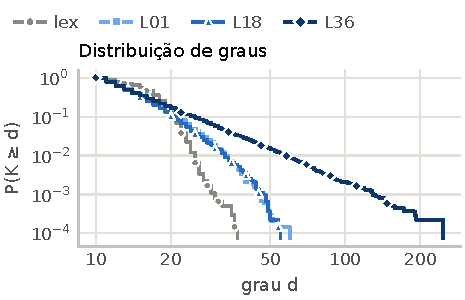
\includegraphics{figuras/graus.pdf}\hfill
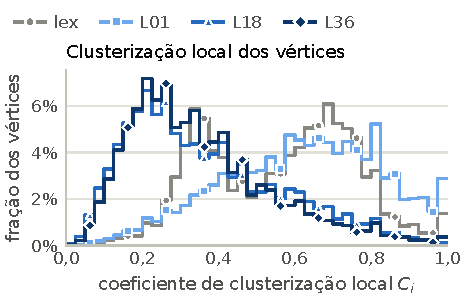
\includegraphics{figuras/clusterizacao_local.pdf}
\caption{À esquerda, a distribuição de graus em escala log-log, como distribuição
acumulada complementar $P(K \ge d)$ (item 7). À direita, a distribuição do coeficiente
de clusterização local $C_i$ (item 3), em 40 faixas de largura 0,025.}
\label{fig:graus-clust}
\end{figure}

\textbf{Clusterização local (item 3, Fig.~\ref{fig:graus-clust}).} Em lex e L01 a
distribuição de $C_i$ se concentra entre 0,5 e 0,85, com um excesso em $C_i=1$ (vértices
cuja vizinhança é um grupo completo). Em L18 e L36 ela se desloca para um pico perto de
0,2 e uma cauda longa. A mudança atinge a maioria dos vértices; não é efeito de um grupo
pequeno.

\textbf{Distribuição de graus (item 7, Fig.~\ref{fig:graus-clust}).} O grau mínimo é sempre
$k=10$. Em lex a cauda é curta (máximo 37); em L01 e L18 ela se alonga (máximos 60 e 55);
em L36 ela se torna pesada, com máximo 247. Esse é o fenômeno de \textit{hubness}: na
camada final, poucas ocorrências são escolhidas como vizinhas por muitas outras. O
fenômeno será estudado na rede direcionada (grau de entrada) no restante do projeto.

\begin{figure}[h]
\centering
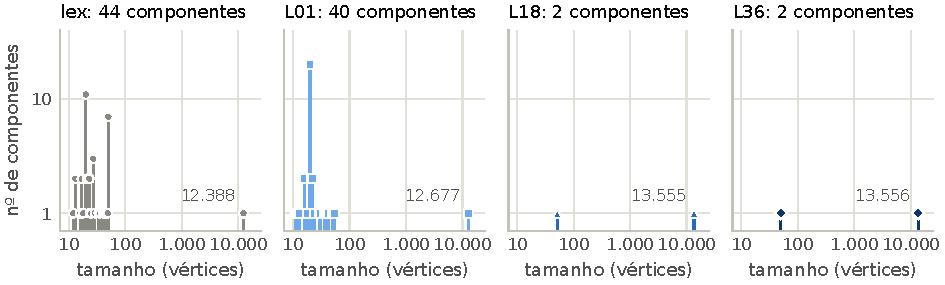
\includegraphics{figuras/componentes.pdf}
\caption{Distribuição dos tamanhos das componentes conexas (item 8). Os rótulos dão o
tamanho da maior componente; os dois eixos estão em escala logarítmica.}
\label{fig:componentes}
\end{figure}

\textbf{Componentes (item 8, Fig.~\ref{fig:componentes}).} As redes lex e L01 têm 44 e 40
componentes. Além da gigante (91\% e 93\% dos vértices), há dezenas de componentes de 10
a 50 vértices, cada uma formada por ocorrências de 1 a 5 tipos de token: por exemplo, as
50 ocorrências de ``ão'' em lex e as 50 de ``para'' em L01. Nelas a identidade lexical
isola grupos inteiros de ocorrências. Em L18 e L36 restam só 2 componentes: a gigante
(99,6\%) e uma de cerca de 50 vértices formada pelas ocorrências na primeira posição da
sequência, cuja representação nessas camadas é muito diferente das demais.

\begin{figure}[h]
\centering
\begin{minipage}[c]{0.49\textwidth}
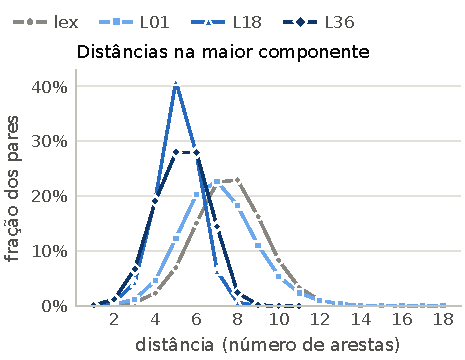
\includegraphics{figuras/distancias.pdf}
\end{minipage}\hfill
\begin{minipage}[c]{0.47\textwidth}
\caption{Distribuição das distâncias entre os pares de vértices da maior componente
(itens 4 e 5). A distância média é a média dessa distribuição, e o diâmetro é o maior
valor com frequência positiva.}
\label{fig:distancias}
\end{minipage}
\end{figure}

\textbf{Distância média e diâmetro (itens 4 e 5, Fig.~\ref{fig:distancias}).} Como lex e
L01 não são conexas, as distâncias são calculadas na maior componente, sobre todos os
pares, por busca em largura a partir de cada vértice. A distância média cai de 7,6 (lex)
e 7,1 (L01) para 5,1--5,3 (L18 e L36), e o diâmetro cai de 18 para 11. Para comparação,
um grafo aleatório com o mesmo tamanho e grau médio teria distância média em torno de
$\ln|V|/\ln\langle d\rangle \approx 3{,}5$. As redes contextuais combinam, portanto,
clusterização muito acima da aleatória com distâncias mais curtas que as da rede lexical.

\textbf{Síntese.} Já nas métricas globais, a passagem lex/L01 $\to$ L18/L36 aparece
como uma reorganização: a clusterização cai, as distâncias encolhem, as componentes
isoladas por token se fundem na componente gigante e surgem \textit{hubs}. Lex e L01 são
muito parecidas, o que sugere que a mudança se concentra entre os blocos 1 e 18. Essa
hipótese será testada no restante do projeto com as medidas por vértice (Jaccard das
vizinhanças, dominância lexical), com as comunidades (NMI com tipo de token e com
contexto) e com a robustez a $k$, à simetrização e ao desempate.

\end{document}
